\chapter{Composants, technologies et outils}  \label{outils}
Ce chapitre décrit tous les composants, technologies et outils nécessaires à la réalisation du projet \textit{Virtual-Vertigo}. Pour chaque section, un exemple d'utilisation général a été inclus. 
%%%%%%%%%%%%%%%%%%%%%%%%%%%%%%%%%%%%%%%%%%%%%%%%%%%%%%%%%%%%%%%%%%%%%%%%%%%%%%%%%%%%%%%%%%%%%%%%%%%%%%%%%%%%%%%%%%%%%%%%%%%

\section{Google CardBoard} \label{cardboard}

Les \textit{Google CardBoard} sont des casques de réalité virtuelle en carton équipé de deux lentilles et dans lesquels peut venir se loger un \textsf{smartphone}. Elles se construisent à la maison avec très peu de matériel et sont accessibles à tout le monde à un prix très bas. Google permet ainsi via ses lunettes de pouvoir utiliser des applications de réalité virtuelle 3D sans avoir à mettre une somme d'argent trop importante.

\subsection*{Version 1}
\begin{figure}[h]
	\centering
		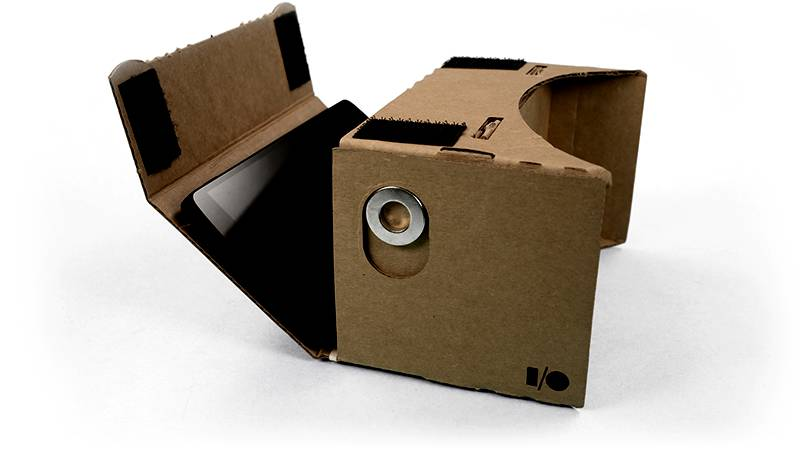
\includegraphics[scale=0.15]{CardBoard1.jpg}
		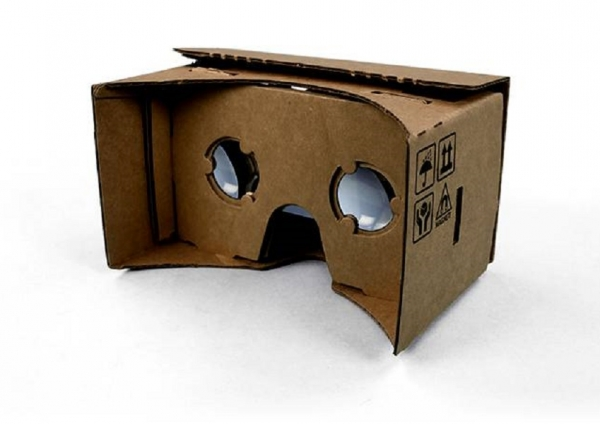
\includegraphics[scale=0.15]{CardBoard1-2.jpg}
	\caption{\label{CardBoard1} Illustrations des \textit{Google CardBoard version 1}}
\end{figure}

La première version des \textit{Google CardBoard} a été introduite en 2014.

\subsubsection{Matériel pour le montage}
Pour la construction, il ne faut pas grand chose :
\begin{itemize}
\item du carton pas trop épais (1-2 millimètres)
\item deux lentilles biconvexes
\item un tag NFC
\item un aimant céramique
\item un aimant néodyme
\item du velcro \\

\end{itemize}

A noter que les aimants servent à interagir avec le \textsf{smartphone} pour actionner les boutons. \\

Les patrons de conception et les instructions de montage sont mis à disposition sur le site des \textit{Google CardBoard} \cite{CardBoard}. Il suffit alors de les imprimer, les coller sur le carton, découper et assembler tout les composants pour obtenir des \textit{Google CardBoard}. Il est également possible d'acheter des \textit{Google CardBoard} pré-fabriquées.\\

Dans le cadre du Projet \textit{Virtual-Vertigo}, les \textit{Google CardBoard} utilisées ont complètement été construites manuellement. Cependant, seules les lentilles biconvexes ont servi. En effet, l'aimant et le patch NFC n'ont pas été utilisé pour \textit{Virtual-Vertigo}.\\

A noter qu'un tutoriel contenant les instructions pour le montage des \textit{Google CardBoard} est disponible en annexe.

\subsection*{Version 2} 
\begin{figure}[h]
	\centering
		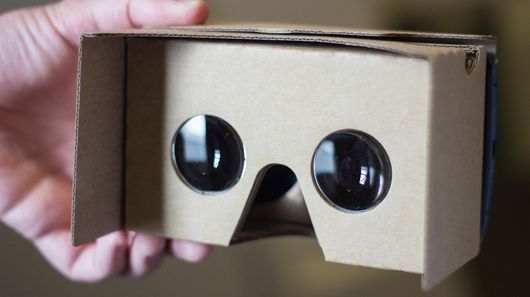
\includegraphics[scale=0.25]{CardBoard2.jpg}
		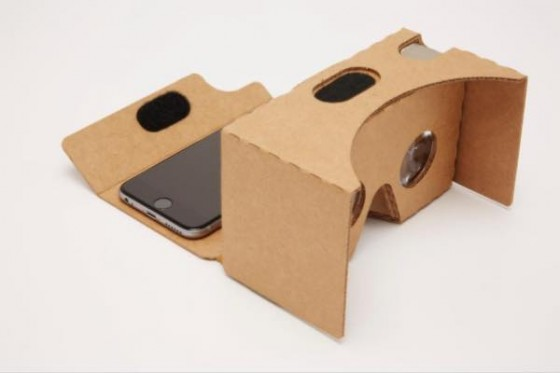
\includegraphics[scale=0.2]{CardBoard2-1.jpg}
	\caption{\label{CardBoard2} Illustrations des Google CardBoard version 2}
\end{figure}
La nouvelle version des Google CardBoard est sortie en juin 2015

\subsubsection{Nouveautés}
\begin{itemize}
	\item Cette version est capable de contenir un \textsf{smartphone} jusqu'à 6 pouces.
	\item Les aimants étant pas fiable sur la version 1 ont été remplacés par un bouton physique interagissant directement avec le \textsf{smartphone}.
	\item Google a implémenté un SDK qui supporte les \textsf{iPhones} et les \textsf{Android}.
	\item Le montage est plus simple.
\end{itemize}

\subsubsection{Matériel pour le montage}
Google n'a pas encore transmis les patrons de conception ni la liste de matériel pour construire cette nouvelle version.

\pagebreak
\subsection*{Vision stéréoscopique sur le smartphone} \label{vision}
La stéréoscopie est une technique mise en oeuvre pour reproduire une perception de 3D à partir de deux images. Elle se base sur le fait que la perception humaine de la 3D se forme dans le cerveau lorsqu'il reconstitue une seule image à partir de la perception de deux images provenant de chaque oeil. \\

La stéréoscopie pour les \textit{Google CardBoard} s'effectue sur le \textsf{smartphone}. La vue affichée sur le \textsf{smartphone} doit avoir une vue pour chaque oeil. Puis c'est par l'intermédiaire des lentilles que ses images planes seront perçues comme des images 3D.

\begin{figure}[H]
\centering 
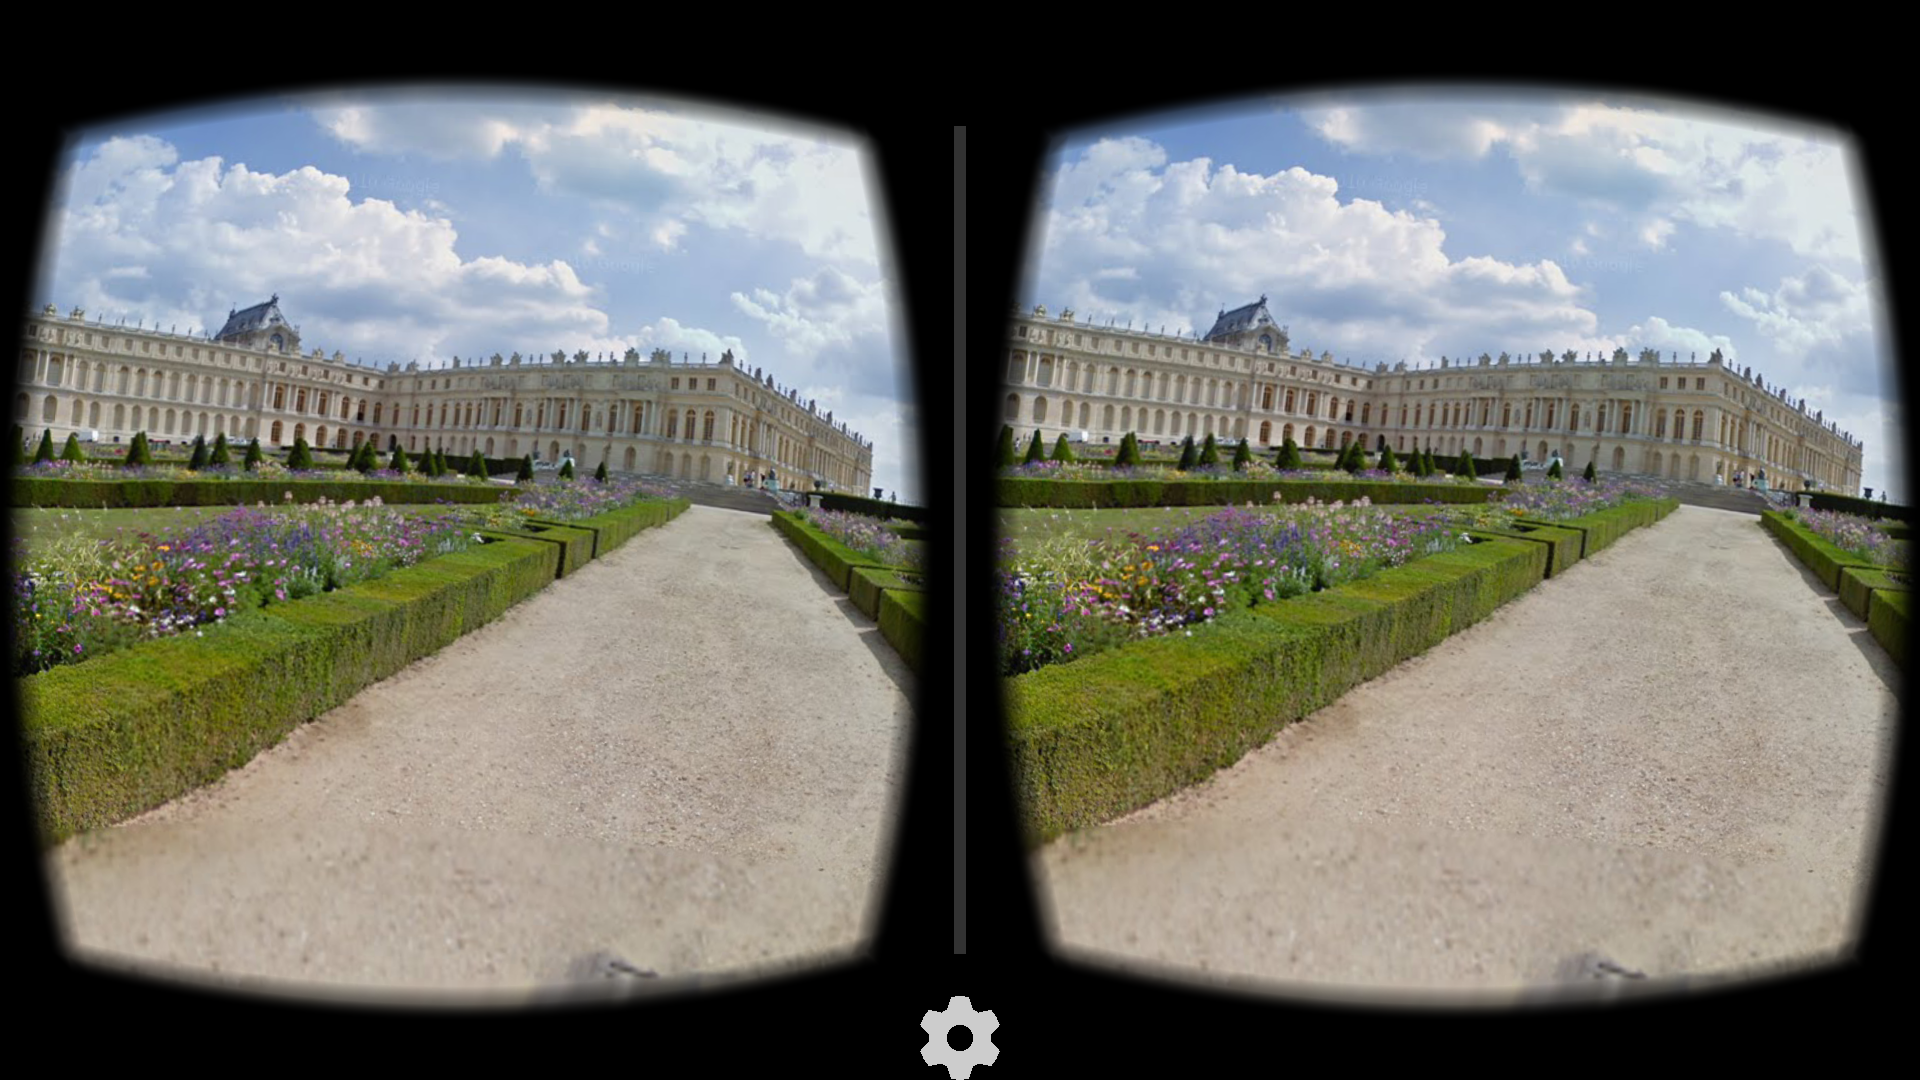
\includegraphics[scale=0.1]{stereoscopie.png}
\caption{\label{sterescopie} Stéréoscopie sur smartphone pour \textit{Google CardBoard}}
\end{figure}

Pour plus d'informations sur la stéréoscopie, voir \cite{stereoscopie}.

\subsection*{Applications sur Google CardBoard}  \label{applications}
La vue sur le \textsf{smartphone} doit absolument être stéréoscopique afin que les lentilles donnent un effet de 3D. Ainsi, en plaçant le \textsf{smartphone} dans les \textit{Google CardBoard} avec une application pour \textsf{CardBoard} lancée, l'immersion dans le monde virtuel est immédiate. \\

Une application utilisant les \textit{Google CardBoard} doit être stéréoscopique et peut par exemple être implémentée en deux langages différents : 
\begin{itemize}
\item comme une application \textsf{Android} en Java : cela implique que tout est stocké et exécuté sur le \textsf{smartphone};
\item comme une application Web via un Framework 3D : cela implique que le \textsf{smartphone} charge seulement une page Web.
\end{itemize}

\subsubsection*{Applications disponibles}  \label{dispo}
Plusieurs applications sont disponible pour les \textit{Google CardBoard} implémentée sur \textsf{Android} ou le Web. Ci-dessous, la description d'une application \textsf{Android} suivi de la description d'une application Web pour les \textit{Google CardBoard}.\\
L'\textsf{application Android CardBoard} disponible sur le play store permet de tester plusieurs démonstrations sur les Google CardBoard. Pour vous procurer l'application \textsf{CardBoard}, voir \cite{androidCardboard}. Ci-dessous la liste des démonstrations que l'application propose : 
\pagebreak
\begin{itemize}
\item \textbf{Earth : } aller où vous voulez avec \textsf{Google Earth};
\item \textbf{Tour Guide : } visiter Versailles avec un guide;
\item \textbf{My Videos : } regarder vos vidéos sur un grand écran;
\item \textbf{Exhibit : } examiner un artefact culturel sous différents angles;
\item \textbf{Photo Sphere : } regarder vos photos sphère;
\item \textbf{Windy Day : } suivre une histoire dans une courte scène interactive de \textsf{Google Spotlight Stories}, votre cinéma de poche (pour plus d'informations sur \textsf{Google Spotlight Stories}, voir \cite{spotlight}).\\

\end{itemize}
L'\textsf{application ClassroomVR} disponible sur internet utilise le \textit{Framework X3DOM} (voir section~\ref{x3dom}). Cette application met en scène une salle de classe stéréoscopique 3D. Ci-dessous une illustration de cette application : 

\begin{figure}[H]
\centering
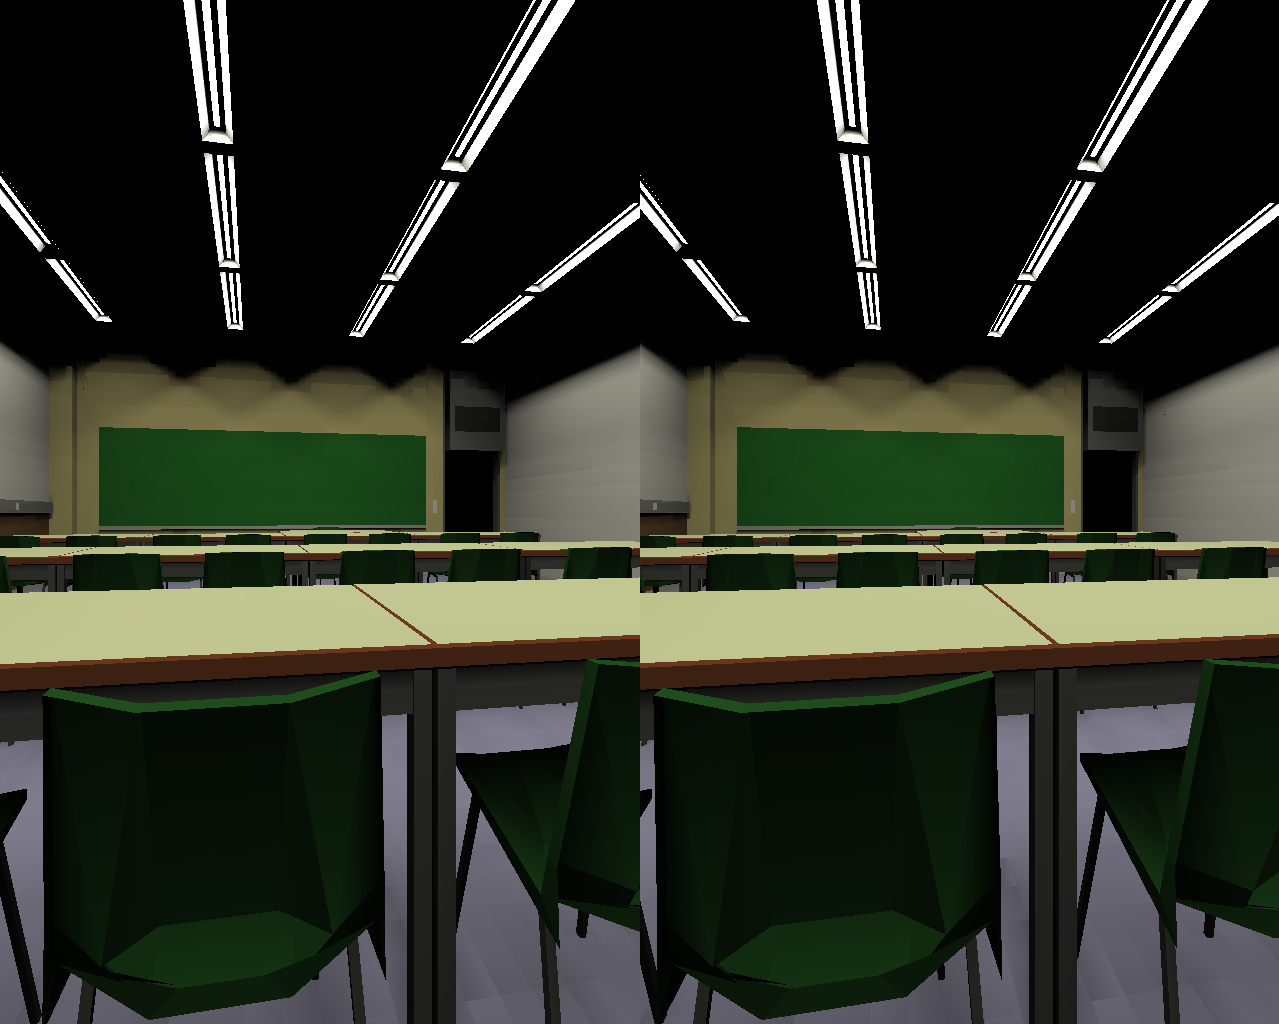
\includegraphics[scale=0.4]{classroom.png}
\caption{\label{classroom} Illustration de l'\textsf{application ClassroomVR}}
\end{figure}
La scène~\ref{classroom} met en scène une salle de classe contenant des tables, des chaises et un tableau noir. Lorsque cette vue est visualisée via les lentilles des \textit{Google CardBoard}, la personne est plongée dans cette salle et peut l'observer depuis un point fixe.


%%%%%%%%%%%%%%%%%%%%%%%%%%%%%%%%%%%%%%%%%%%%%%%%%%%%%%%%%%%%%%%%%%%%%%%%%%%%%%%%%%%%%%%%%%%%%%%%%%%%%%%%%%%%%%%%%%%%%%%%%%%
 
\pagebreak 
\section{Kinect version 1}  \label{kinect}
Le \textit{Kinect} est un périphérique initialement destiné à la \textsf{console de jeux Xbox 360}. Il permet à l'utilisateur d'interagir en utilisant son corps plutôt qu'une manette. Depuis quelques années, Microsoft a mis à disposition un SDK permettant d'utiliser le \textit{Kinect} sur un ordinateur Windows. Cependant, le Kinect nécessite des caractéristiques hardware spécifiques (pour plus d'informations sur les caractéristiques du\textit{ Kinect v1}, voir~\cite{PrerequisKinectv1}).\\

Le \textit{Kinect} a été choisi pour capter et reporter les mouvements et le déplacement de la personne. Ainsi grâce au \textit{Kinect}, la personne peut voir ses mains ou ses pieds (en simplifié) lorsqu'il avance sur la planche. Le \textit{Kinect version 1} a été choisi en particulier car l'école disposait déjà d'un tel appareil et également parce qu'il convenait amplement aux besoins de \textit{Virtual-Vertigo}.\\

A noter qu'un tutoriel contenant les instructions pour l'installation et l'utilisation du \textit{Kinect v1} est disponible en annexe.

\subsection{Composants et caractéristiques}  \label{composant}
Cette section contient une description succincte des composants et caractéristiques du \textit{Kinect v1}.
\begin{figure}[h]
	\centering
		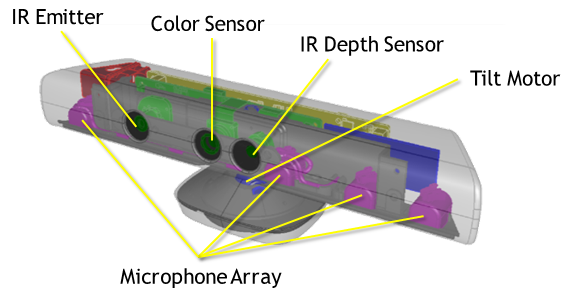
\includegraphics[scale=0.5]{SpecKinect.png}
	\caption{\label{SpecKinect} Structure du \textit{Kinect version 1}}
\end{figure}

\begin{itemize}
	\item \textbf{Color Sensor : } caméra RGB
	\item \textbf{IR Emitter : } émet des infrarouges pour le Depth Sensor
	\item \textbf{IR Depth Sensor : } lit les infrarouges retournés au Kinect, puis les convertis en information de 	profondeur mesurant la distance entre l'objet et le Kinect
	\item \textbf{Tilt Motor : } permet de changer et de déterminer l'orientation du \textit{Kinect v1} sur un axe 3D
	\item \textbf{Microphone Array : } 4 microphones qui permettent de capturer le son\\
\end{itemize}

\begin{center}
	\begin{tabular}{| l | c |}
	\hline
		\textbf{Max Distance} & ~4.5 m \\ \hline
		\textbf{Min Distance} & 0.8 m (normal mode) and 0.4 m (near mode)\\ \hline
		\textbf{Horizontal Field Of View} & 57 degrees \\ \hline
		\textbf{Vertical Field Of View} & 43 degrees \\ \hline
		\textbf{Frame Rate} & 30 fps \\ \hline
		\textbf{Skeleton Joints Defined} & 20 \\ \hline
		\textbf{Full Skeleton Tracked} & 2 \\ \hline
		\textbf{Audio Format} & 16 kHz (24 bit mono PCM) \\ \hline
		\textbf{Vertical Tilt Range} & +- 27 degrees \\
		\hline
	\end{tabular}
	\captionof{table}{\label{spec} Tableau illustrant les caractéristiques du \textit{Kinect v1}}
\end{center}


\subsubsection{Comparaison v1 et v2}

\begin{figure}[h]
	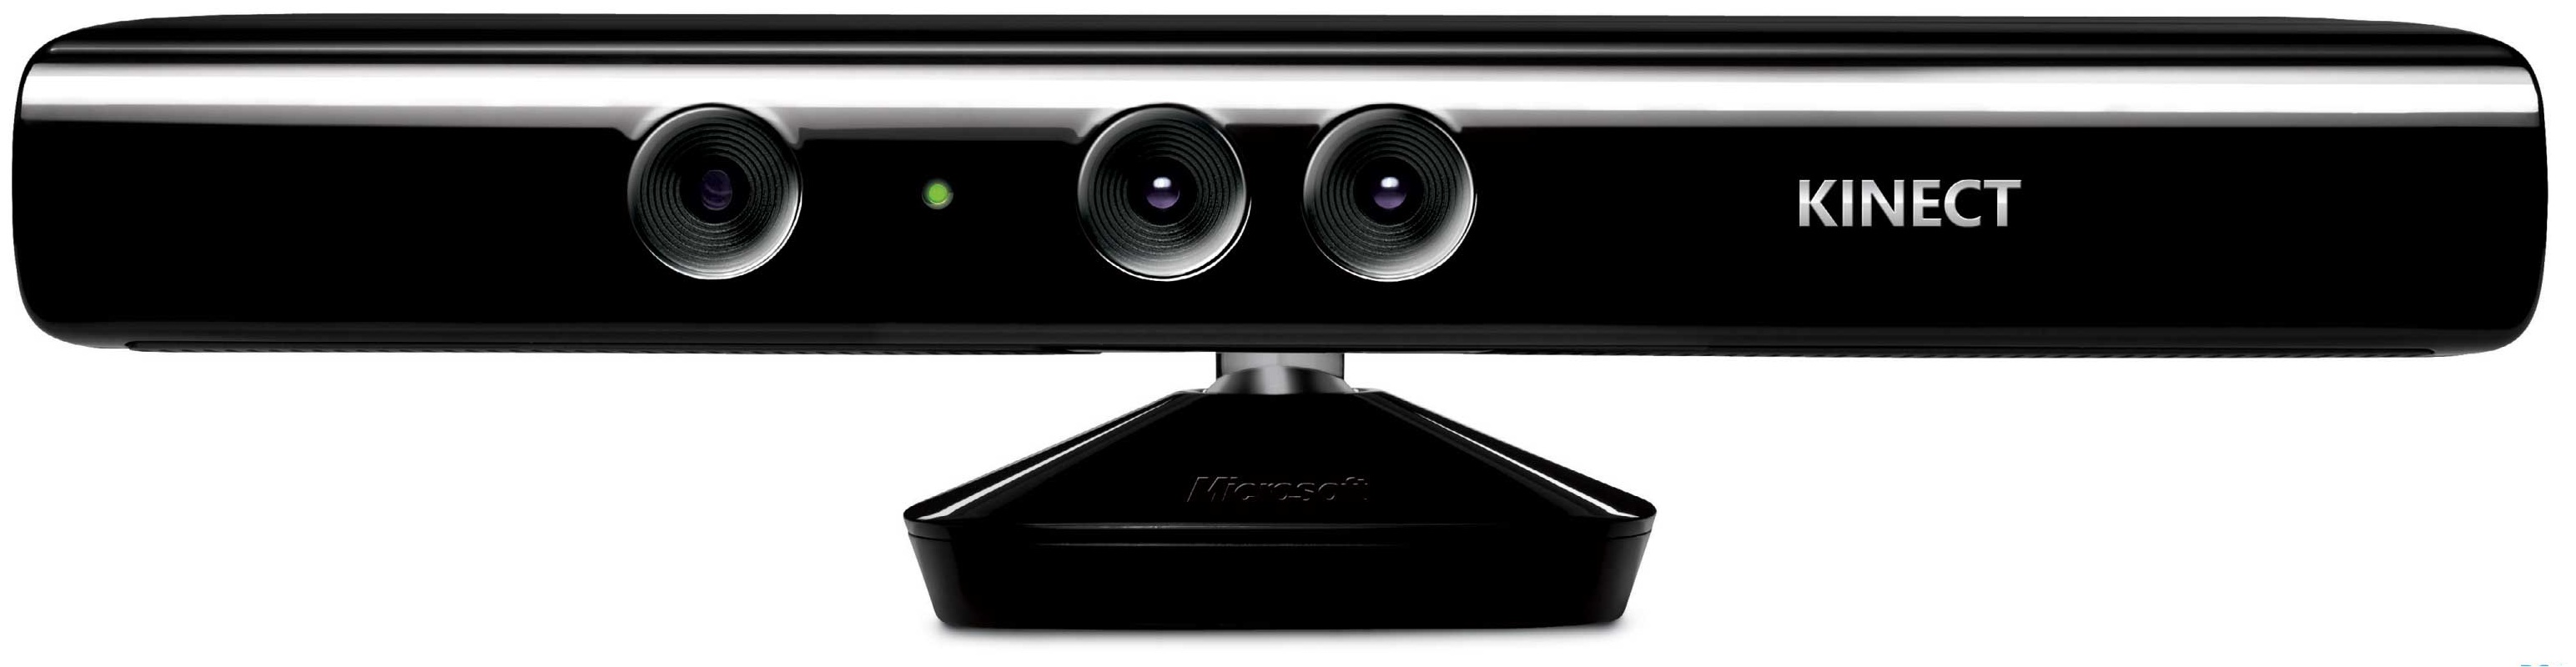
\includegraphics[scale=0.1]{Kinectv1.jpeg}
	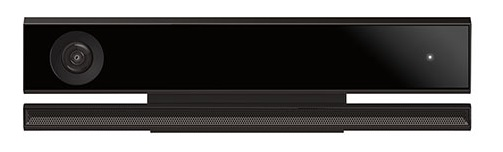
\includegraphics[scale=0.5]{Kinectv2.jpg}
	\caption{\label{Kinectv1v2} Kinect v1 vs Kinect v2}
\end{figure}
\begin{itemize}
	\item la plus grande différence entre les 2 versions est la résolution.\\
	 La résolution couleur est plus de 3 fois plus élevée et la résolution de profondeur est quasiment 2 fois plus élevée.
	\item les champs de vue horizontal et vertical ont également augmenté. 
	\item 25 articulations sont captées par le \textit{Kinect v2} contre 20 pour le \textit{Kinect v1}.
	\item le principal défaut du \textit{Kinect v2} est que les caractéristiques hardware sont plus exigeantes.
	\item le nombre de fps (Frame par secondes) n'a pas changé entre les 2 versions. 
\end{itemize}

\subsection{Capture des données}
Le \textit{Kinect} permet de capter différents types de données d'une personne de plusieurs manières. Les différentes captures se font en utilisant les capteurs du \textit{Kinect}.\\

Le \textit{Kinect} permet de capturer les données d'une personne dans 2 positions différentes : \textsf{default}, la personne est debout, et \textsf{seated}, la personne est assise. Les informations ci-dessous peuvent être capturés dans les deux positions. 
\pagebreak
\subsubsection{Angle de vue}
Le \textit{Kinect} capte les informations sur un rayon de 43 degrés à la verticale et de 57 degrés à l'horizontale. L'angle de vue du \textit{Kinect} se traduit comme un cône, le \textit{Kinect} étant la partie la plus étroite du cône.\\

Ci-dessous une illustration des angles de vue du \textit{Kinect}.
\begin{figure}[H]
	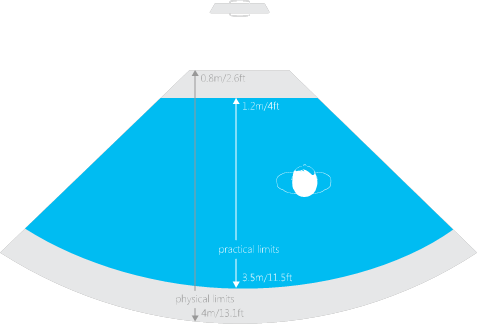
\includegraphics[scale=0.5]{fieldviewHorizontal.png}
	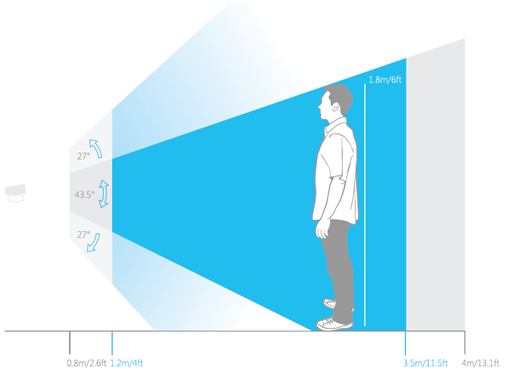
\includegraphics[scale=0.5]{fieldviewVertical.png}
	\caption{\label{AngleVue} Angles de vue du \textit{Kinect} horizontal et vertical}
\end{figure}

\subsubsection{Color Stream}
Le \textsf{Color Stream} sert de caméra RGB au \textit{Kinect}. Il retransmet les informations que le \textsf{Color Sensor} capte. Il permet donc d'afficher et de modifier la vue en temps réel. \\

Il permet d'utiliser plusieurs formats différents :  
\begin{itemize}
\item Raw YUV, résolution de $640\times 480$ à 15 fps 
\item RGB, résolution de $1280\times 960$ à 12 fps
\item RGB, résolution de $640\times 480$ à 30 fps
\item YUV, résolution de $640\times 480$ à 15 fps
\item Infrared de type MONO16, résolution de $640\times 480$ à 30 fps permet de capter en cas de lumière faible
\item RawBayer de type MONO8, résolution de $1280\times 960$ à 12 fps ou  de $640\times 480$ à 30 fps pour utiliser son propre algorithme de reconstruction d'image
\end{itemize}
Le \textsf{Color Sensor} n'est pas utilisé dans ce projet.

\subsubsection{Depth Stream}
Le \textsf{Depth Stream} sert à capter les informations en utilisant la profondeur détectée par les infrarouges. Il permet donc d'afficher et de modifier le vue en profondeur avec des nuances de gris.
Il capte la profondeur en deux modes : \textsf{default}, de 0.6 à 4m, et \textsf{near}, de 0.4 à 3m. \\
Il permet également de le faire à 30 fps en différentes dimensions : $640\times 480$, $320\times 240$ et $80\times 60$.\\ 
Le \textsf{Depth Stream} n'est pas utilisé dans ce projet.

\pagebreak
\subsubsection{Skeletal Stream}
Le \textsf{Skeletal Stream} retourne les positions du squelette ainsi que la position, en 3 dimensions, de chacune des 20 articulations de référence sur le squelette en mètres (voir section~\ref{articulation}). \\
Il faut savoir que l'origine est le \textit{Kinect}, que les axes x et y sont les offset du centre de vision du \textit{Kinect} et que l'axe z est la distance entre le \textit{Kinect} et l'objet.\\

\begin{figure}[H]
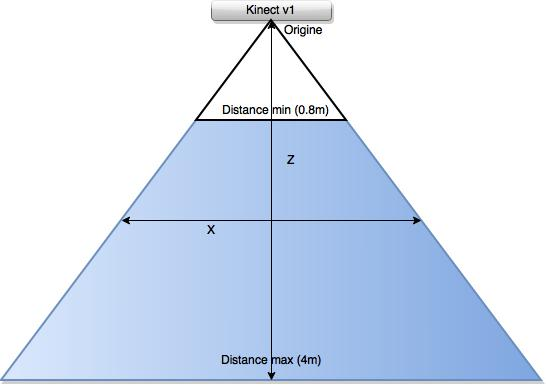
\includegraphics[scale=0.4]{SkeletonX.jpg}
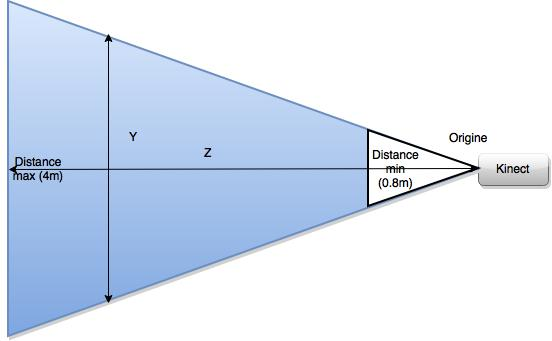
\includegraphics[scale=0.4]{SkeletonY.jpg}
\caption{\label{positions} Illustration des axes par rapport au \textit{Kinect}}
\end{figure}
Le figure~\ref{positions} illustre comment sont placé les axes x, y et z en fonction du \textit{Kinect}. La partie verte sur chaque figure correspond à la zone que le \textit{Kinect} capte.


\subsection{Articulations du squelette et leurs orientations} \label{articulation} 
\begin{figure}[h]
	\centering
		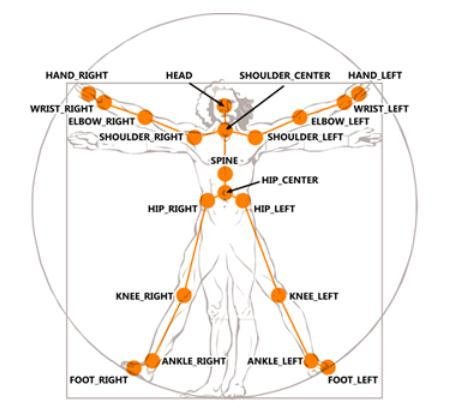
\includegraphics[scale=0.47]{squelette.jpg}
	\caption{\label{Joints} Articulations du squelette captés par le Kinect}
\end{figure}
Les 20 articulations que le \textit{Kinect v1} détecte se trouvent sur l'illustration~\ref{Joints}. A chacune de ces articulations correspond un identifiant qui permet ensuite de retrouver le nom de l'articulation détectée. Le tableau~\ref{valeurs} ci-dessous donne ces valeurs.
\begin{center}
	\begin{tabular}{| c | c | c |}
	\hline
		\textbf{Identifiant} & \textbf{Articulation} & \textbf{Nom sur squelette} \\ \hline
		0 & base of the spine & hipcenter \\ \hline
		1 & middle of the spine & spine \\ \hline
		2 & neck & shouldercenter \\ \hline
		3 & head & head \\ \hline
		4 & left shoulder & shoulderleft \\ \hline
		5 & left elbow & elbowleft \\ \hline
		6 & left wrist & wristleft \\ \hline
		7 & left hand & handleft \\ \hline
		8 & right shoulder & shoulderleft \\ \hline
		9 & right elbow & elbowright \\ \hline
		10 & right wrist & wristright \\ \hline
		11 & right hand & handright \\ \hline
		12 & left hip & hipleft \\ \hline
		13 & left knee & kneeleft \\ \hline
		14 & left ankle & ankleleft \\ \hline
		15 & left foot & footleft \\ \hline
		16 & right hip & hipright \\ \hline
		17 & right knee & kneeright \\ \hline
		18 & right ankle & ankleright \\ \hline
		19 & right foot & footright \\ \hline
		20 & spine at the shoulder & n'est pas détecté \\ \hline
		21 & tip of the left hand & n'est pas détecté \\ \hline
		22 & left thumb & n'est pas détecté \\ \hline
		23 & tip of the right hand & n'est pas détecté \\ \hline
		24 & right thumb & n'est pas détecté \\
		\hline
	\end{tabular}
\captionof{table}{\label{valeurs} Tableau illustrant les valeurs de chaque articulation}
\end{center}

Le \textit{Kinect v1} capture également l'orientation des articulations du squelette. Connaître l'orientation des articulations du squelette permet d'effectuer une plus précise animation d'un avatar. Le \textit{Kinect v1} peut capter l'orientation de deux manières : la rotation hiérarchique, basé sur les membres reliés, et l'orientation absolue, utilisant les coordonnées de la caméra. \\

Les deux images ci-dessous illustrent comment le \textit{Kinect v1} capture l'orientation des articulations du squelette :
\begin{figure}[H]
\centering
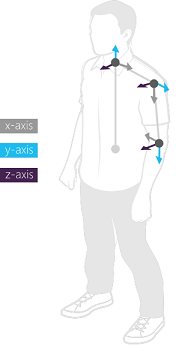
\includegraphics[scale=0.6]{hierachical.png}
\caption{\label{hierachical} Illustration de la rotation hiérachique}
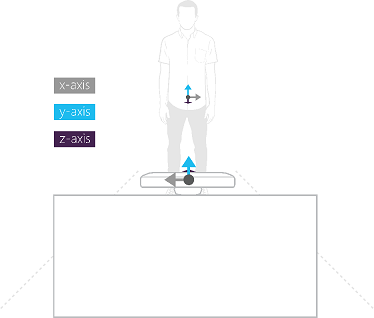
\includegraphics[scale=0.6]{absolute.png}
\caption{\label{absolute} Illustration de l'orientation absolue}
\end{figure}
Pour plus d'informations sur les orientations des articulations, voir \cite{jointOrientation}.
Ces données d'orientations peuvent être retournées sous forme de quaternions ou de matrices de rotations. Ci-dessous une illustration des deux formes : 
\begin{equation}
q = r + x\textbf{j}  + y\textbf{j} + z\textbf{k}
\end{equation}
\begin{center}
tel que r est un réel consistant la partie réelle  et x\textbf{i} + y\textbf{j} + z\textbf{k} consistant la partie pure d'Hamilton, où : \textbf{i} = (1,0,0),\textbf{j} = (0,1,0), \textbf{k} = (0,0,1).
\end{center}

\begin{figure}[H]
\centering
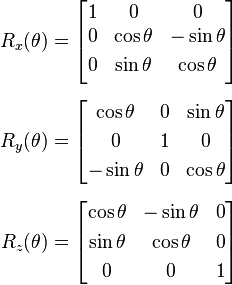
\includegraphics[scale=0.5]{matriceRotation.png}
\caption{\label{hierachical} Illustration des matrices de rotations en x, y et z}
\end{figure}

Pour plus d'informations sur les quaternions, voir \cite{quaternion} et pour plus d'informations sur les matrices de rotations, voir \cite{matrice}.


\subsection{Outils utilisés dans le projet}  \label{outilsUtilise}

\subsubsection{Framework .NET}
Le \textit{Framework .NET} est utilisé par Windows. Il s'appuie sur une norme CLI (Common Language Infrasture) qui est indépendante du langage de programmation. Cela permet aux langages compatibles respectant cette norme d'avoir accès à toutes les bibliothèques disponibles sur l'environnement d'exécution. Il fournit une approche unifiée pour la conception d'applications Windows et Web.

\subsubsection{Visual Studio 2013}
\textit{Visual Studio 2013} est un logiciel de développement pour Windows conçue par Microsoft. Il permet de générer des applications Web ASP.NET, des services Web XML et bien d'autres. \\
Les langages tel que \textit{Visual Basic, Visual C++, Visual C\# et Visual J\#} permettent de mieux tirer parti des fonctionnalités du \textit{Framework .NET}.


\subsubsection{SDK 1.8 du Kinect v1}
Le \textit{SDK 1.8 pour Windows} fournit des outils et une API pour implémenter une application utilisant le \textit{Kinect}. \\

Le \textit{SDK 1.8} est la mise à jour des anciens SDK. En plus des autres SDK, il contient :
\begin{itemize}
	\item \textbf{Kinect Background Removal :} fournit un écran vert pour une seule personne.
	\item \textbf{Webserver for Kinect Data Streams : }permet l'envoi des informations captées par le \textit{Kinect} sur une page Web utilisant les \textit{WebSockets}.
	\item \textbf{Color Capture and Camera Pose Finder for Kinect Fusion :} permet de scanner un objet 3D puis de le modéliser en utilisant le \textit{Kinect}.
	\item Beaucoup d'exemples.
\end{itemize}
Pour plus d'informations sur les différents \textit{SDK du Kinect v1}, Voir \cite{SDKKinectv1}.  \\

Ce SDK est le dernier que Windows a sorti pour le \textit{Kinect v1}. Quand le \textit{Kinect v2} est sorti le SDK 2.0 a pris le relais. \\

\pagebreak
\paragraph{Exemple d'utilisation \\ }
L'exemple qui suit capte la personne devant le Kinect. Il est séparé en deux parties : l'initialisation du \textit{Kinect} et la capture des données.

\lstset{language=[Sharp]C,
basicstyle=\footnotesize,
backgroundcolor=\color{backcolour}, 
captionpos=b,
frame=lines, % Oberhalb und unterhalb des Listings ist eine Linie
showspaces=false,
showtabs=false,
breaklines=true,
showstringspaces=false,
breakatwhitespace=true,
escapeinside={(*@}{@*)},
commentstyle=\color{greencomments},
morekeywords={partial, var, value, get, set},
keywordstyle=\color{bluekeywords},
stringstyle=\color{redstrings}
}
\begin{lstlisting}
//Initialisation du Kinect
KinectSensor kinect = null;

void StartKinectST()
{
	// Get first Kinect Sensor
	kinect = KinectSensor.KinectSensors.FirstOrDefault(s => s.Status == KinectStatus.Connected); 
	kinect.SkeletonStream.Enable(); // Enable skeletal tracking
	
	// Allocate ST data
	skeletonData = new Skeleton[kinect.SkeletonStream.FrameSkeletonArrayLength]; 

	// Get Ready for Skeleton Ready Events
	kinect.SkeletonFrameReady += new EventHandler<SkeletonFrameReadyEventArgs>(kinect_SkeletonFrameReady); 

	// Start Kinect sensor
	kinect.Start(); 
}

//Capture des donnees
private void kinect_SkeletonFrameReady(object sender, SkeletonFrameReadyEventArgs e)
{
  // Open the Skeleton frame
  using (SkeletonFrame skeletonFrame = e.OpenSkeletonFrame()) 
  {
  	// check that a frame is available
	if (skeletonFrame != null && this.skeletonData != null) 
	{
	  // get the skeletal information in this frame
	  skeletonFrame.CopySkeletonDataTo(this.skeletonData);
	  
	  // draw the skeletons
	  foreach (Skeleton skeleton in this.skeletonData)
      {
          if (skeleton.TrackingState == SkeletonTrackingState.Tracked)
          {
              DrawSkeletonPosition(skeleton.Position);
          }
      } 
	}
  }
}

\end{lstlisting}

\subsubsection{Socket IO C\# Client}
\textit{Socket IO C\# Client} (socket.io-csharp-client) est un projet disponible sur \textit{GitHub} \cite{SocketIOCSharp}. Il permet de faire communiquer un programme C\# avec un \textit{serveur NodeJS}. Il utilise le \textsf{package} \textit{NuGet}, un gestionnaire de \textsf{packages} sur \textit{Visual Studio}. Il permet d'ajouter des \textsf{packages} à une application \textit{Visual Studio}. \\
Il permet de créer et modifier des \textsf{packages} et fournit un grand nombre de \textsf{packages} pour Windows. \\
Il utilise également \textit{WebSocket4Net}, un autre projet \textit{GitHub} \cite{WebSocket4Net} qui permet d'utiliser les \textit{WebSockets} client.\\

Ce projet est utilisé pour transmettre les données captées au client HTML. Il a permis de résoudre le problème décrit au chapitre~\ref{problemes}

\paragraph{Exemple d'utilisation \\ }
L'exemple ci-dessous n'utilise pas le \textit{Kinect}. Il montre comment utiliser \textit{SocketIOC\# Client} dans un projet.

\lstset{language=[Sharp]C,
basicstyle=\footnotesize,
backgroundcolor=\color{backcolour}, 
captionpos=b,
frame=lines, % Oberhalb und unterhalb des Listings ist eine Linie
showspaces=false,
showtabs=false,
breaklines=true,
showstringspaces=false,
breakatwhitespace=true,
escapeinside={(*@}{@*)},
commentstyle=\color{greencomments},
morekeywords={partial, var, value, get, set},
keywordstyle=\color{bluekeywords},
stringstyle=\color{redstrings}
}

\begin{lstlisting}
using System;
using SocketIO.Client;

namespace SimpleClient
{   
   class Example
   {
      static void Main()
      {
         var io = new SocketIOClient();

         var socket = io.Connect("http://localhost:3000/");

         socket.On("data", (args, callback) =>
         {
            Console.WriteLine("Server sent:");

            for (int i = 0; i < args.Length; i++)
            {
               Console.WriteLine("[" + i + "] => " + args[i]);
            }
         });

         string line;

         while ((line = Console.ReadLine()) != "q")
         {
            socket.Emit("data", line);
         }
      }
   }
}
\end{lstlisting}


%%%%%%%%%%%%%%%%%%%%%%%%%%%%%%%%%%%%%%%%%%%%%%%%%%%%%%%%%%%%%%%%%%%%%%%%%%%%%%%%%%%%%%%%%%%%%%%%%%%%%%%%%%%%%%%%%%%%%%%%%%%

\pagebreak
\section{Technologies 3D}  \label{technologies}
Ce projet nécessite la visualisation de scènes 3D et la modélisation de scènes 3D. Le \textit{Framework X3DOM} permet à ce projet de ne pas être dépendant du système d'exploitation du \textsf{smartphone} car il suffit d'un accès internet. Cette solution permet à n'importe qui de pouvoir facilement tester et utiliser ce projet. Il permet également d'avoir plusieurs clients, un testeur et une visionner. \\ 

Les logiciels de modélisations 3D \textit{Blender et Cinema4D} ont été utilisés pour modéliser des scènes 3D. \textit{Blender} permet d'exporter les scènes 3D en format X3D supporté par \textit{X3DOM}. Le personnage 3D a été modélisé en utilisant le logiciel \textit{MakeHuman}. Plus d'informations sur la modélisation des scènes du projet au chapitre~\ref{implementation}.

\subsection{X3DOM}  \label{x3dom}
\begin{figure}[H]
\flushright
   
\includegraphics[scale=0.2]{x3domLogo.png}
\end{figure}

\textit{X3DOM} est un \textsf{Framework} open source qui permet d'afficher des scènes 3D sur une page Web. \textit{X3DOM} est la composition entre \textsf{X3D} (Extensible 3D Graphics) et \textsf{DOM} (Document Object Model). Il permet d'intégrer X3D dans le DOM et d'utiliser, par exemple un listener d'événements ou les modifications du HTML dynamiquement avec \textsf{JavaScript}. \\

L'utilisation de \textit{X3DOM} au lieu d'une autre librairie apporte certains avantages :
\begin{itemize}
\item pas besoin d'un plugin pour afficher les scènes 3D;
\item étant basé sur un nouveau profil HTML de l'ISO Standard X3D, il est conforme au standard;
\item il existe une large communauté de développeurs;
\item utilisation du HTML et DOM plutôt que d'apprendre à programmer avec une nouvelle API;
\item il suffit de télécharger et inclure les documents CSS et \textsf{JavaScript} pour l'utiliser.\\
Pour plus d'informations sur \textit{X3DOM} voir \cite{X3DOM}, sur X3D voir section~\ref{x3d} ou sur DOM voir \cite{DOM}.

\end{itemize}

\paragraph{Exemple d'utilisation \\ }
Afin d'ajouter de la 3D sur une simple page HTML, il faut impérativement avoir les éléments suivants : 

\begin{itemize}
\item le fichier de script x3dom.js permettant de manipuler la 3D,
\item le fichier de style x3dom.css pour le placement des éléments dans la scène 3D.\\

\end{itemize}
\pagebreak
Voici un exemple très simple d'utilisation de \textit{X3DOM}. Dans cet exemple, un cône, un cube et une sphère sont créés sur la même ligne et bougent tous en même temps.

\lstset{style=mystyle} 
\begin{lstlisting}[language=Html]
<html> 
   <head>
    <meta http-equiv="X-UA-Compatible" content="IE=edge"/> 
     <title>My first X3DOM page</title> 
     <script src='http://www.x3dom.org/download/x3dom.js'> </script> 
     <link rel='stylesheet' type='text/css' 
           href='http://www.x3dom.org/download/x3dom.css'/> 
   </head> 
   <body> 
	 <x3d width='500px' height='400px'> 
	   <scene> 
		<shape> 
		   <appearance> 
			 <material diffuseColor='1 0 0'></material> 
		   </appearance> 
		   <box></box> 
		</shape> 
		<transform translation='-3 0 0'> 
		  <shape> 
			 <appearance> 
			   <material diffuseColor='0 1 0'></material> 
			 </appearance> 
			 <cone></cone> 
		  </shape> 
		</transform> 
		<transform translation='3 0 0'> 
		  <shape> 
			 <appearance> 
			   <material diffuseColor='0 0 1'></material> 
			 </appearance> 
			 <sphere></sphere> 
		  </shape> 
		</transform> 
	   </scene> 
	</x3d> 
   </body> 
</html> 
\end{lstlisting}

Voici le résultat de cet exemple : 
\begin{figure}[H]
\centering
	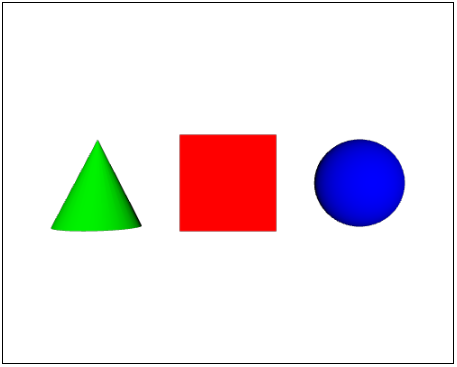
\includegraphics[scale=0.5]{exempleX3DOM.png}
\end{figure}

\subsection{Logiciels 3D - Blender, MakeHuman et Cinema4D}  \label{logiciel3D}

\subsubsection{Blender}
\textit{Blender} est un logiciel de modélisation, d'animation et de rendu 3D développé par la \textsf{Fondation Blender}. \\
\textit{X3DOM} prévoit une balise utilisant un format que seul \textit{Blender} met à disposition en exportation au format X3D. 

\subsubsection{Format x3d} \label{x3d}
Le \textit{format X3D} (Extensible 3D) est un format de fichier graphique et multimédia orienté 3D.\\
X3D s'appuie sur une structure de type graphe de scène. \\
X3D est un couplage entre une page HTML et un objet \textit{Blender} \\
Le format X3D est très similaire à \textit{X3DOM}. Un exemple du format X3D et un exemple de \textit{X3DOM} sont placés en annexes afin de voir la comparaison (pour plus d'informations sur X3D voir \cite{X3D}).

\subsubsection{MakeHuman}
\textit{MakeHuman} est un logiciel libre de modélisation 3D de corps humains. Les modèles générés sont destinés à être utilisés sur \textit{Blender} ou un autre logiciel 3D. \\

Il dispose d'une interface simple permettant de créer facilement un corps humain de n'importe quel type et en modifiant et personnalisant toutes les caractéristiques du corps humain.

\subsubsection{Cinema4D}
\textit{Cinema4D} est un logiciel de création 3D développé par \textsf{Maxon}. Il permet la modélisation, le texturage, l'animation et le rendu d'objets 3D.

%%%%%%%%%%%%%%%%%%%%%%%%%%%%%%%%%%%%%%%%%%%%%%%%%%%%%%%%%%%%%%%%%%%%%%%%%%%%%%%%%%%%%%%%%%%%%%%%%%%%%%%%%%%%%%%%%%%%%%%%%%%

\pagebreak 
\section{Serveur Web Virtual-Vertigo en NodeJS}  \label{serveur}
Dans le cadre de ce projet, un serveur est nécessaire pour transmettre les informations captées par le \textit{Kinect} aux clients HTML. \\

\begin{figure}[H]
	\centering
		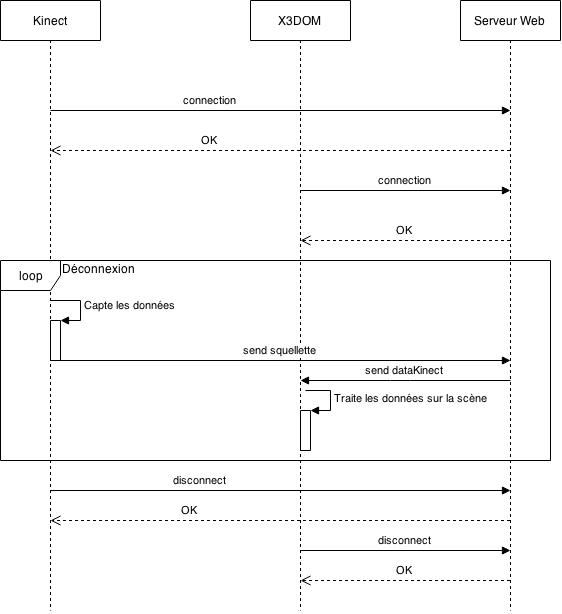
\includegraphics[scale=0.7]{DiagrammeServeur.jpg}
	\caption{\label{DiagrammeServeur} Diagramme de séquences illustrant la communication avec le serveur}
\end{figure}
Comme vous pouvez le voir sur ce diagramme de séquences~\ref{DiagrammeServeur}, le \textit{Kinect} et le client HTML se connectent au serveur. Puis le \textit{Kinect} envoie toutes les secondes les informations captées et dès que le serveur reçoit les données du \textit{Kinect}, il les retransmet directement aux clients HTML qui va les interpréter sur la scène 3D. Tout ceci s'effectue jusqu'à la déconnexion du \textit{Kinect} et des clients HTML.\\

Le \textit{serveur Web Virtual-Vertigo} est un serveur Web utilisant les \textit{WebSockets} pour les communications. Lors du projet de semestre sur le même thème, un travail préliminaire a permis de choisir entre \textit{MeteorJS} et \textit{NodeJS}. \textit{MeteorJS} est un \textsf{Framework} permettant de construire des sites Web modernes et d'implémenter automatiquement un serveur Web, sans avoir besoin de gérer quoi que ce soit. Cependant, \textit{NodeJS} a été choisi car on avait besoin de plus de contrôle sur l'implémentation du serveur.\\
Pour plus d'informations sur les \textit{WebSockets} voir \cite{websocket}, sur \textit{MeteorJs} voir \cite{MeteorJS}.

\subsection{NodeJS}
\begin{figure}[H]
	\flushright
   		
\includegraphics[scale=0.1]{nodeLogo.png}
\end{figure}
\textit{NodeJS} est un \textsf{Framework} logiciel et évènementiel en \textsf{JavaScript}. Il contient une bibliothèque de serveur HTTP, ce qui permet de faire tourner et de mieux contrôler un serveur Web sans avoir besoin d'un logiciel externe. \\
L'avantage de ce \textsf{Framework} est qu'il permet d'ajouter plusieurs modules permettant de manipuler les services Web plus facilement (par exemple l'utilisation de \textit{WebSockets} avec le module \textit{Socket.io}). Ces modules sont disponibles car il utilise \textit{npm}, un gestionnaire de \textsf{packages} officiel pour \textit{NodeJS} qui permet d'installer des applications disponibles sur le dépôt \textit{npm}. \\
A noter que la plupart des projets disponibles sur le dépôt \textit{npm} sont des projets implémentés par un utilisateur qui a voulu partager son travail en le mettant à disposition sur \textit{GitHub} (our plus d'informations sur \textit{NodeJS}, voir \cite{NodeJS}).

\paragraph{Exemple d'utilisation \\}
NodeJS contient deux modules déjà installés :
\begin{itemize}
\item http : module permettant de créer un serveur \textit{http}
\item net : module permettant de créer un serveur \textit{tcp\\}

\end{itemize}

L'exemple qui suit met en place un serveur en utilisant le module http. 

\lstset{style=mystyle} 
\begin{lstlisting}[language=JavaScript]
// Load the http module to create an http server.
var http = require('http');

// Configure our HTTP server to respond with Hello World to all requests.
var server = http.createServer(function (request, response) {
  response.writeHead(200, {"Content-Type": "text/plain"});
  response.end("Hello World\n");
});

// Listen on port 8000, IP defaults to 127.0.0.1
server.listen(8000);

// Put a friendly message on the terminal
console.log("Server running at http://127.0.0.1:8000/");
\end{lstlisting}


A noter qu'un tutoriel contenant les instructions pour l'installation et l'utilisation de \textit{NodeJS} et \textit{npm} est disponible en annexe.

\subsection{Module ExpressJS}
ExpressJS installé avec npm, permet de créer et gérer une application Web plus facilement parce qu'il s'occupe de création du serveur, il suffit donner une adresse ip et il le crée pour nous. Dans ce projet, il est utilisé gérer les parties accessibles depuis le serveur. L'utilisation d'ExpressJS a permis de mettre en place l'architecture décrite dans le chapitre précédent.\\

\paragraph{Exemple d'utilisation \\}
L'exemple suivant crée un serveur local sur le port 3000. Lorsqu'un client se connecte, un message \textsf{Hello World} lui est transmis.\\

\lstset{style=mystyle} 
\begin{lstlisting}[language=JavaScript]
var express = require('express');
var app = express();

app.get('/', function (req, res) {
  res.send('Hello World!');
});

var server = app.listen(3000, function () {

  var host = server.address().address;
  var port = server.address().port;

  console.log('Example app listening at http://%s:%s', host, port);

});
\end{lstlisting}


\subsection{Module Socket.io}
Pour ce projet, les \textit{WebSockets} ont été choisis car ils permettent de communiquer et de partager des données avec plusieurs clients HTML. En effet, pour ce projet, le serveur Web devait recevoir et envoyer des données aux clients sans les traiter. En général l'inverse est utilisé, c'est le client qui transmet des données au serveur qui les traitent. Les \textit{WebSockets} ont permis d'envoyer et de recevoir des données depuis le serveur sans avoir a effectuer un traitement préalable. \\

\textit{Socket.io} est un module installé par npm permettant d'utiliser les \textit{WebSockets}. Il permet de facilement les manipuler que ce soit du côté client ou du côté serveur. Dans ce projet, l'utilisation de \textit{SocketIOC\# Client} a nécessité d'utiliser la version 0.9 de \textit{Socket.io}. \textit{SocketIOC\#} permet d'utiliser les \textit{WebSockets} afin de se connecter et d'envoyer ses informations captées par le \textit{Kinect} puis de renvoyer au client HTML. Le module \textit{Socket.io} utilise une syntaxe précise qui doit être respectée du côté client et du côté serveur: 
\begin{itemize}
\item lancement du serveur (seulement pour le serveur) : \texttt{io.listen(\textit{adresse ip du serveur});}
\item l'attente de connexions (seulement pour le serveur) : \texttt{io.sockets.on('connection', \\
function(socket)$\{$ \textit{réception et envoi de données}$\});$}
\item connexion au serveur (seulement pour le client) : \texttt{socketIO.connect(\textit{adresse ip et port du serveur});}
\item la réception de données : \texttt{socket.on(\textit{label de l'envoi}, function(data)$\{$\textit{traitement des données reçue}$\});$}
\item l'envoi de données : \texttt{socket.emit(\textit{label de l'envoi}, \textit{données});}
\end{itemize}
Pour plus d'informations, voir \cite{SocketIO}.\\

\paragraph{Exemple d'utilisation \\}
L'exemple suivant est un chat entre les clients connectés. Cet exemple utilise également le module \textit{ExpressJS} parce que la transmission des messages entre les clients est gérée par un serveur. Lors de la réception d'un message, le serveur le transmet à tous les clients connectés. \\
Cet exemple contient deux parties, un client HTML et un serveur.

\lstset{style=mystyle} 
\begin{lstlisting}[language=JavaScript]
\\ Serveur
var app = require('express')();
var http = require('http').Server(app);
var io = require('socket.io')(http);

app.get('/', function(req, res){
  res.sendFile(__dirname + '/index.html');
});

io.on('connection', function(socket){
  socket.on('chat message', function(msg){
    io.emit('chat message', msg);
  });
});

http.listen(3000, function(){
  console.log('listening on *:3000');
});
\end{lstlisting}


\lstset{style=mystyle} 
\begin{lstlisting}[language=Html]
\\ Client HTML
<!doctype html>
<html>
  <head>
    <title>Socket.IO chat</title>
    <script src="https://cdn.socket.io/socket.io-1.2.0.js"></script>
    <script src="http://code.jquery.com/jquery-1.11.1.js"></script>
  </head>
  <body>
    <ul id="messages"></ul>
    <form action="">
      <input id="m" autocomplete="off" /><button>Send</button>
    </form>
    <script>
      var socket = io();
      $('form').submit(function(){
        socket.emit('chat message', $('#m').val());
        $('#m').val('');
        return false;
      });
      socket.on('chat message', function(msg){
        $('#messages').append($('<li>').text(msg));
      });
    </script>
  </body>
</html>
\end{lstlisting}
